In the previous chapters, we presented the motivation of this work, the literature review showing the main concepts behind work, then, we breifly described some related works. In this chapter, we will describe the problem, the whole experimentation setupp and the tools used to accomplish the proposed objectives.

\section{Database}

The first necessary task is to find a database spread over several years. For this, the Neural Information Processing Systems database was chosen, \cite{nipsweb}. With 7241 entries spread in a thirty-years range, this base contains academic papers from the NIPS conference, one of the most prestigious yearly events in the machine learning community. The Table \ref{tab:dataset-description} contains the description of the main columns present in the data set.

\begin{table}[h!]
	\centering
	\caption{Main feature description for NIPS data set.}
	\label{tab:dataset-description}
	\begin{tabular}{r|lc}
		    Feature & Description          & Data Type \\ \hline
		         id & Paper identifier     &  Integer  \\
		       year & Year of publication  &  Integer  \\
		      title & Title of publication &   Text    \\
		   abstract & Publication abstract &   Text    \\
		paper\_text & Publication corpus   &   Text
	\end{tabular}
\end{table}

\section{Pre-processing the Data}

With the chosen database, we must define a data pre-processing pipeline to normalize the documents, putting all of then at the same pattern. For this, we can use the normalization techniques shown in Chapter \ref{chap:literature} like stemming, lemmatization, stop words removal, and all necessary textual manipulations to obtain the best text representation for the documents.

\subsection{Normalization Pipeline}

To be more specific about the normalization process, let us describe it in more details. First of all, we must concatenate the title, the abstract and the paper text to treat all the paper information like a single document in our corpus. Done that, we proceed with the other normalization steps in the order as follows.

\begin{enumerate}
	\item \textbf{Drop links:} drop all possible links, by regular expression, in the text that could might disturb the others steps;
	\item \textbf{Remove numbers:} remove all numbers, by regular expression, in the text;
	\item \textbf{Expand contractions:} Convert some english contractions into their full form;
	\item \textbf{Remove punctuation:} Replace all punctuation marks to empty space;
	\item \textbf{Convert special characters:} Replace special characters, accented letters for example, with their ASCII form;
	\item \textbf{Case convertion:} Change all characthers by thei lower forms;
	\item \textbf{Lemmatization:} Convert the words to their root form by lemmatizing them according their part of speech tag;
	\item \textbf{Remove stop-words:} Remove the english well-known stop words.
\end{enumerate}

Figure \ref{fig:normalized-text} illustrates an example of the application of the above mentioned language processing techniques to a given input.

\begin{figure}[h!]
	\centering
	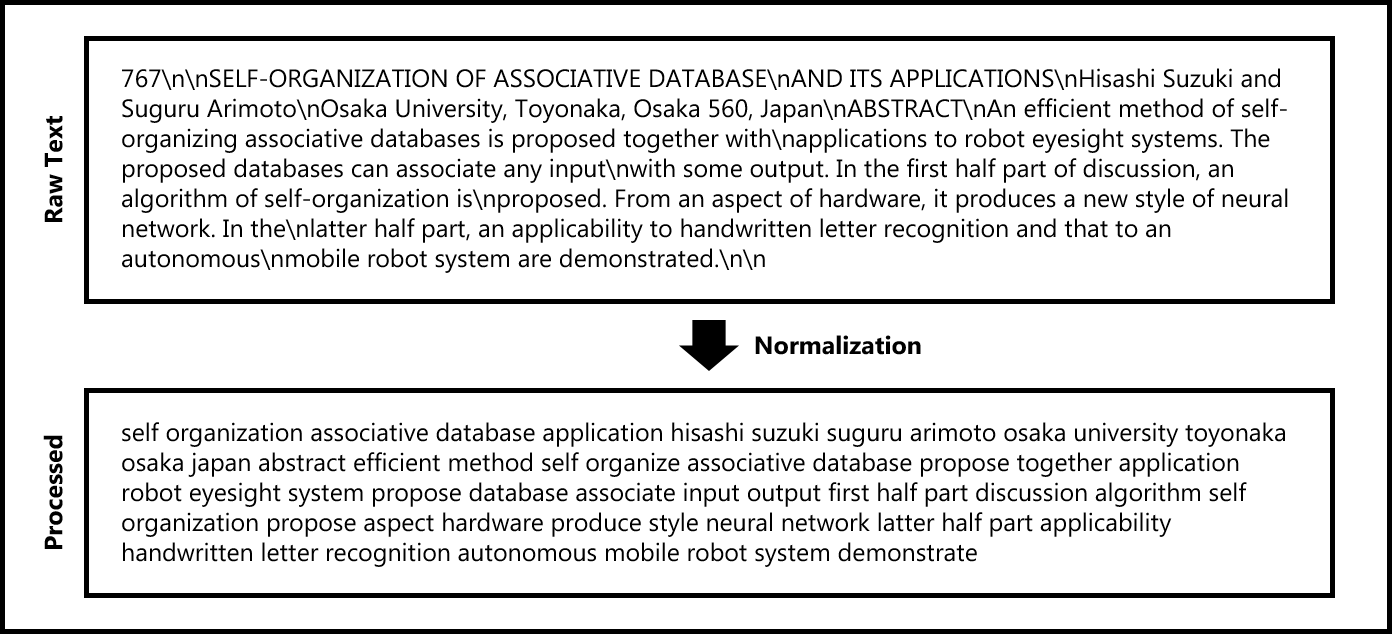
\includegraphics[width=\linewidth]{01.Chapters/04.Materials/normalization-process}
	\caption{Demonstration about the normalization process.}
	\label{fig:normalized-text}
\end{figure}

\subsection{Segmentation}

After processing the data, we need to index then over the time and, then, split the full treated data set in three subsets. They must be time ordered, as shown in Figure \ref{fig:database}, this means that for each document in $T_{i}$ its time index $t_{x}^{(i)}$ must be lower then any index $t_{x}^{(m)}$ in a document contained in $T_{m}$, and so on.

\begin{figure}[h!]
	\centering
	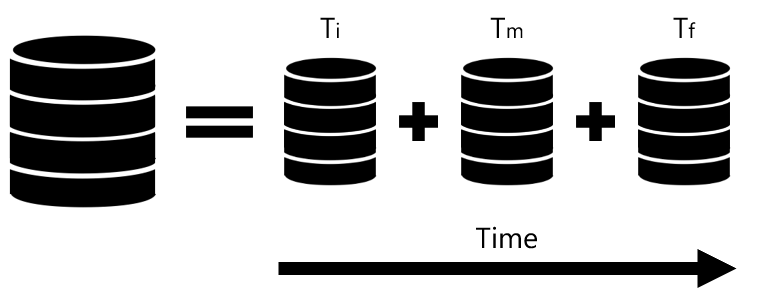
\includegraphics[width=0.5\linewidth]{01.Chapters/04.Materials/database}
	\caption{Database time split representation.}
	\label{fig:database}
\end{figure}

Before proceeding, let us give a name to the subsets. The initial subset will be called \textit{Past} from now on, the middle and final ones will be respectively designated by \textit{Present} and \textit{Future}. To segment these three subsets, let us first analyze the yearly distribution of documents. Figure \ref{fig:yearly-histogram} shows how the documents are spread over the years, and Figure \ref{fig:yearly-cumulative} shows the cumulative distribution of documents with the percentiles marks of 40\% and 80\%.

\begin{figure}[h!]
	\begin{subfigure}{0.45\textwidth}
		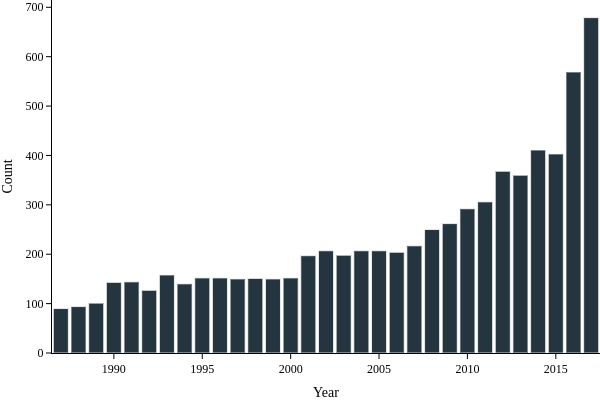
\includegraphics[width=\linewidth]{01.Chapters/04.Materials/yearly-histogram}
		\caption{Histogram for year distribution.} \label{fig:yearly-histogram}
	\end{subfigure}%
	\hfill
	\begin{subfigure}{0.45\textwidth}
		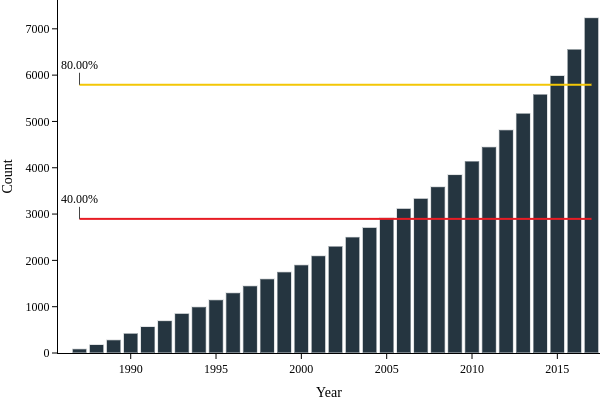
\includegraphics[width=\linewidth]{01.Chapters/04.Materials/yearly-cumulative}
		\caption{Cumulative histogram.} \label{fig:yearly-cumulative}
	\end{subfigure}%
	\caption{Yearly distribution of documents.} 
	\label{fig:yearly-distribution}
\end{figure}

After this division, shown in Figure \ref{fig:yearly-distribution}, we approach the limits to 2004 and 2014. Then, the temporal division for the subsets was done as indicated in the Table \ref{tab:database-description}.

\begin{table}[h!]
	\centering
	\caption{Subsets description after segmentation.}
	\label{tab:database-description}
	\begin{tabular}{r|cc}
		 Subset & No. of documents &    Years    \\ \hline
		   Past &       2713       & 1987 - 2004 \\
		Present &       2877       & 2005 - 2014 \\
		 Future &       1651       & 2015 - 2017
	\end{tabular}
\end{table}

\section{Topic Modeling}

With the \textit{Past} set, techniques of topic modeling will be applied to identify the discussed subjects in the documents. Figure \ref{fig:topic-identification} illustrates the sequence of steps for this task. Next to the topic identification we will obtain a topic set, then each document contained in \textit{Past} can be labeled with at least one topic from the set, this new database will be called by \textit{labeled Past}.

\begin{figure}[h!]
	\centering
	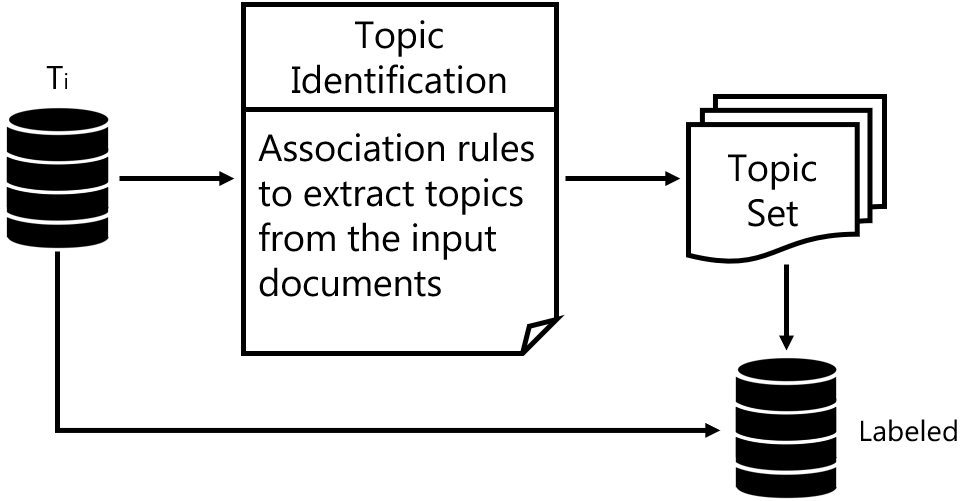
\includegraphics[width=0.7\linewidth]{01.Chapters/04.Materials/topic-identification}
	\caption{Topic identification process.}
	\label{fig:topic-identification}
\end{figure}

% Descrever detalhes de implementação do topic modeling
	% Feature selection - corte de luhn para formação do vocabulario

% Otimização de hiperparâmetros
	% Escolha baseado na coerência

% Rotulagem de dados

% Associação de tópicos passado / presente
	% Modelagem de cada no vocabulário próprio
	% Intercessão de vocabulário
	% Top N matching
	% Global matching
	

\section{Document Classification}

For each topic in our set of discovered topics, we must be able to identify which topics are covered by a new document. Thus, we will build a classifier to perform this verification. Knowing that a document can talk about several topics, so we must have a multi-class classifier. We can see this as an individual binary classifier for each topic that tells us whether the document has it. Using the \textit{labeled Past} set it is possible to build this classifier. Figure \ref{fig:document-classification} illustrates it in detail.

\begin{figure}[h!]
	\centering
	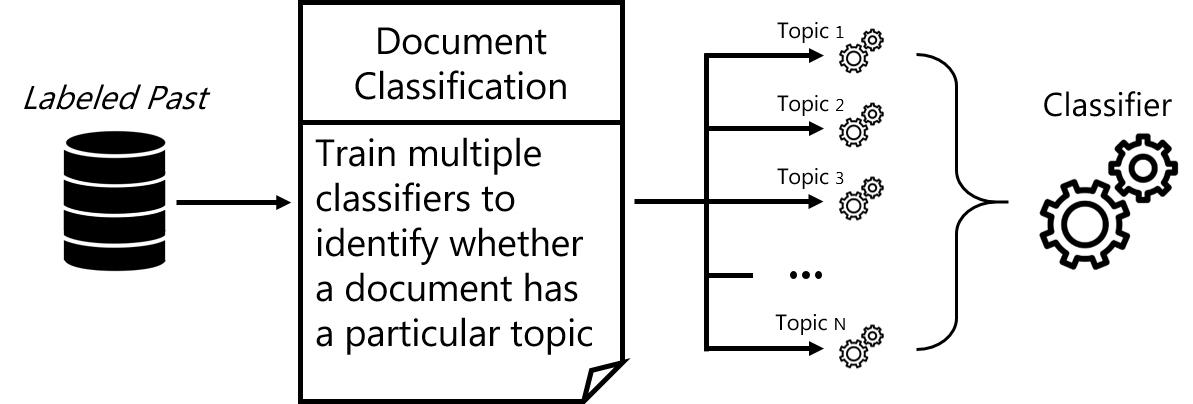
\includegraphics[width=0.9\linewidth]{01.Chapters/04.Materials/document-classification}
	\caption{Multi-class classifier from \textit{Labeled} set.}
	\label{fig:document-classification}
\end{figure}

% Vetorização com vocabulario do passado
	% BoW
	% TF-IDF
	% Word2VEC

% Treinamento do modelo
	% Naive Bayes
	% SVM
	
% Avaliação dos modelos
	% Métricas por validação cruzada
	% Verificação de principais features (palavras) para decidir por determinado tópico
	
% Aplicação do modelo nos dados do presente

% Comparação da classificação



\section{Tools}

In order to execute this steps, some packages and tools were used. Let's briefly describe these tools used so far.

% Gensim
% Spacy
% NLTK
% Sklearn
% Pandas
% Plotly
% Unidecode
% Contractions
% Inflect
% Regex

%\subsection{Forecast evaluation}
%
%Finally, to evaluate the time series model is the last task to be accomplished. Following the flowchart shown in Figure \ref{fig:forecast}, first, we have to label the \textit{Modeler} and \textit{Validation} sets. Then, using labeled \textit{Identifier} and \textit{Modeler} we will build a topic incidence matrix over the time, to apply a forecaster process for those time series. With the labeled \textit{Validation} set we will perform an evaluation for our model and then make conclusions about it.
%
%\begin{figure}[h!]
%	\centering
%	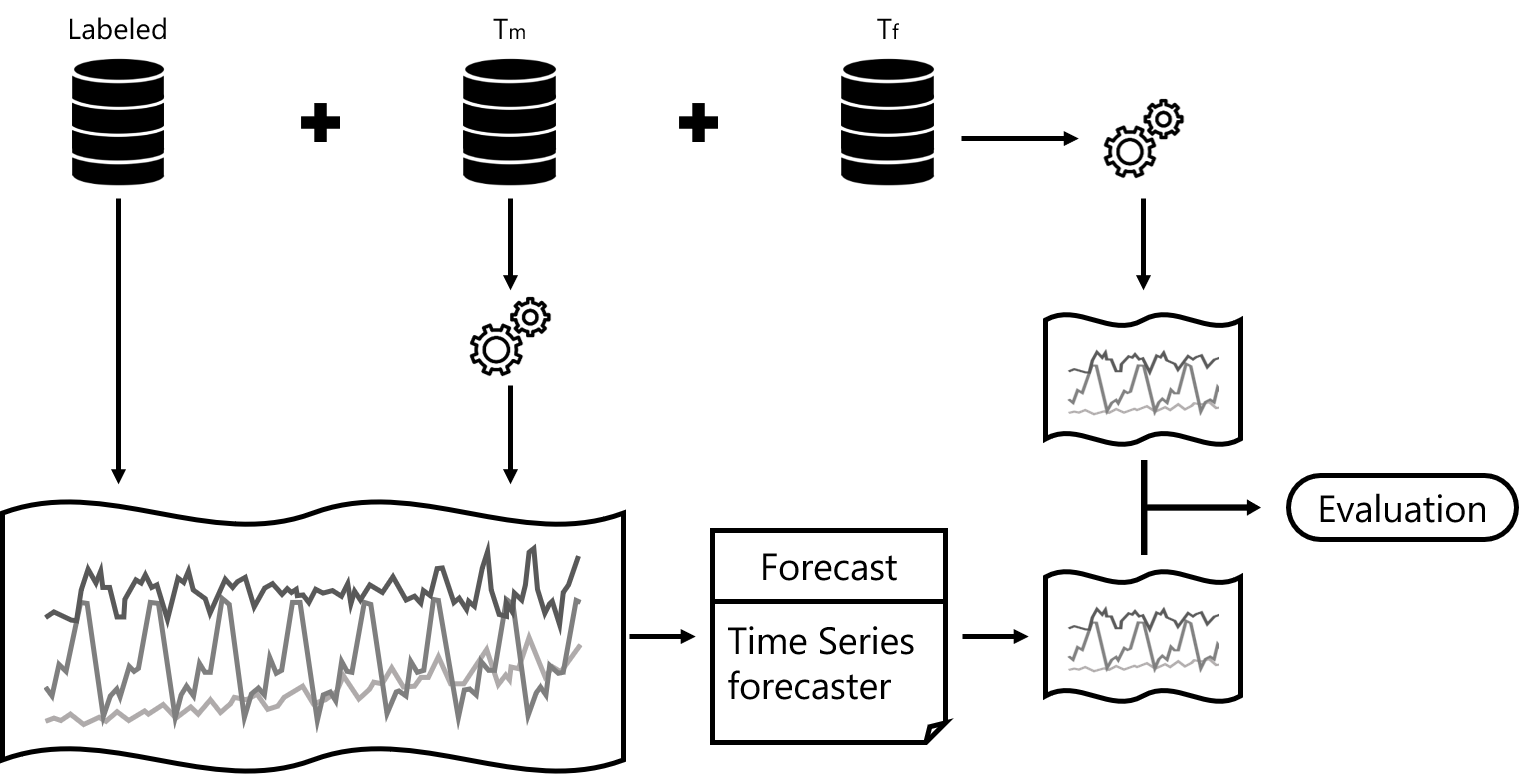
\includegraphics[width=\linewidth]{01.Chapters/04.Materials/forecast}
%	\caption{Flowchart to evaluate the time series model.}
%	\label{fig:forecast}
%\end{figure}
